\title{Multiplexers}
\begin{document}
\section{Tri-state Devices}
\begin{frame}{Three state buffers/inverters}
  \begin{itemize}
    \item Three-state buffers and inverters behave just as regular buffers and inverters do.
    \item They provide a second input, that allows them to be on or off.
    \item The off state causes their output to be in a high impedence state, effectively disconnected from the circuit.
  \end{itemize}
  \begin{center}
    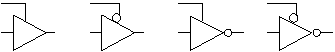
\includegraphics{TriStateLogic}
  \end{center}
\end{frame}

These can be used in combination with a decoder to enable or disable part of a circuit that does not have an explicit enable input. \\
A Bidirectional bus uses a pair of these back to back - see page 422 of the text.

\section{Multiplexers}

\begin{frame}{Multiplexers}
  \begin{definition}
    A \alert{multiplexer} (or mux) connects one of $n$ inputs (each $b$ bits wide) to its $b$ outputs.
  \end{definition}
  \begin{center}
    \includegraphics{multiplexer}
  \end{center}
\end{frame}

\subsection{MSI Multiplexers}

\begin{frame}{74x151 and 74x157}
  \begin{columns}
    \begin{column}{5cm}
      \begin{center}
        \includegraphics{74x151Schematic}
      \end{center}
    \end{column}
    \begin{column}{5cm}
      \begin{center}
        \includegraphics{74x157Schematic}
      \end{center}
    \end{column}
  \end{columns}
\end{frame}

\subsection{Demultiplexers}

\begin{frame}{Demultiplexers}
  In the same way that we may want to select one of many inputs, we may need to apply that input to one of many devices.
  \begin{definition}
    A \alert{demultiplexer} (or dmux) performs the inverse operation of a multiplexer.
  \end{definition}
  \begin{center}
    \includegraphics{MuxDmux}
  \end{center}
\end{frame}

\begin{frame}{74x138 as a demux}
  \begin{center}
    \includegraphics{74x138DMuxSchematic}
  \end{center}
\end{frame}
\end{document}
